\documentclass{beamer}
\usepackage{pgfpages}
\usepackage[backend=bibtex]{biblatex}
\usepackage{multicol}
\usepackage{multimedia}
\usepackage[absolute,overlay]{textpos}
\usepackage{parskip}
\usepackage{hyperref}
\usepackage{lmodern}
\usepackage{bbding}
\usepackage[absolute,overlay]{textpos}
\usepackage{framed} %Used to shade important equations, color devined with shadecolor
\hypersetup{colorlinks=true, urlcolor=blue}
\setlength{\parskip}{\smallskipamount}
\colorlet{shadecolor}{cyan}
%\usepackage[texcoord,grid,gridunit=mm,gridcolor=red!10,subgridcolor=green!10]{eso-pic} %DELETE when done with grid
\setbeameroption{hide notes} % Only slides
%\setbeameroption{show only notes} % Only notes
%\setbeameroption{show notes on second screen=right} % Both
%\bibliography{../../papers/references.bib}
\setbeamerfont{footnote}{size=\tiny}
%\AtEveryCitekey{\clearfield{title}}

%
% Choose how your presentation looks.
%
% For more themes, color themes and font themes, see:
% http://deic.uab.es/~iblanes/beamer_gallery/index_by_theme.html
%
\mode<presentation>
{
\usetheme{Warsaw}      % or try Darmstadt, Madrid, Warsaw, ...
\usecolortheme{default} % or try albatross, beaver, crane, ...
\usefonttheme{default}  % or try serif, structurebold, ...
\setbeamertemplate{navigation symbols}{}
\setbeamertemplate{caption}[numbered]
} 

\usepackage[english]{babel}
%\usepackage[utf8x]{inputenc} %Doesn't play well with biblatex
\usepackage{amssymb}
\usepackage{bm}
\usepackage{color}
\usepackage{graphicx}
\setbeamercovered{invisible}
\setbeamercovered{%
again covered={\opaqueness<1->{100}}} %This changes the opaqueness of each bullet

\newcommand{\red}[1]{{\color{red}{#1}}}
\newcommand{\checkH}[2]{\begin{textblock*}{1cm}(#1,#2){\Huge \red{\Checkmark}}\end{textblock*}}
\newcommand{\checkh}[2]{\begin{textblock*}{1cm}(#1,#2){\huge \red{\Checkmark}}\end{textblock*}}
\newcommand{\checkL}[2]{\begin{textblock*}{1cm}(#1,#2){\Large \red{\Checkmark}}\end{textblock*}}
\newcommand{\checkl}[2]{\begin{textblock*}{1cm}(#1,#2){\large \red{\Checkmark}}\end{textblock*}}
\renewcommand{\rm}[1]{\mathrm{#1}}

\title[{\color{white}{Chapters 4.4-6}}]{Physics 121: \\ Circular Motion}
\author{Cody Petrie}
\institute{Mesa Community College}
\date{}

\begin{document}

%\setbeamertemplate{frametitle}[default][center]
\begin{frame}
\titlepage
\end{frame}

% Uncomment these lines for an automatically generated outline.
%\begin{frame}{Outline}
%  \tableofcontents
%\end{frame}

% Commands to include a figure:
%\begin{figure}
%\includegraphics[width=\textwidth]{your-figure's-file-name}
%\caption{\label{fig:your-figure}Caption goes here.}
%\end{figure}

\begin{frame}{Quiz}
\begin{enumerate}
   \item Which of these accelerations will always cause an object to change direction?
   \begin{columns}
      \begin{column}{0.5\textwidth}
      \begin{enumerate}
         \item[A.] $\vec{a}_x$
         \item[C.] $\vec{a}_\perp$
      \end{enumerate}
      \end{column}
      \begin{column}{0.5\textwidth}
      \begin{enumerate}
         \item[B.] $\vec{a}_y$
         \item[D.] $\vec{a}_\parallel$
      \end{enumerate}
      \end{column}
   \end{columns}
   \item This acceleration will cause the particle to
   \begin{center}
     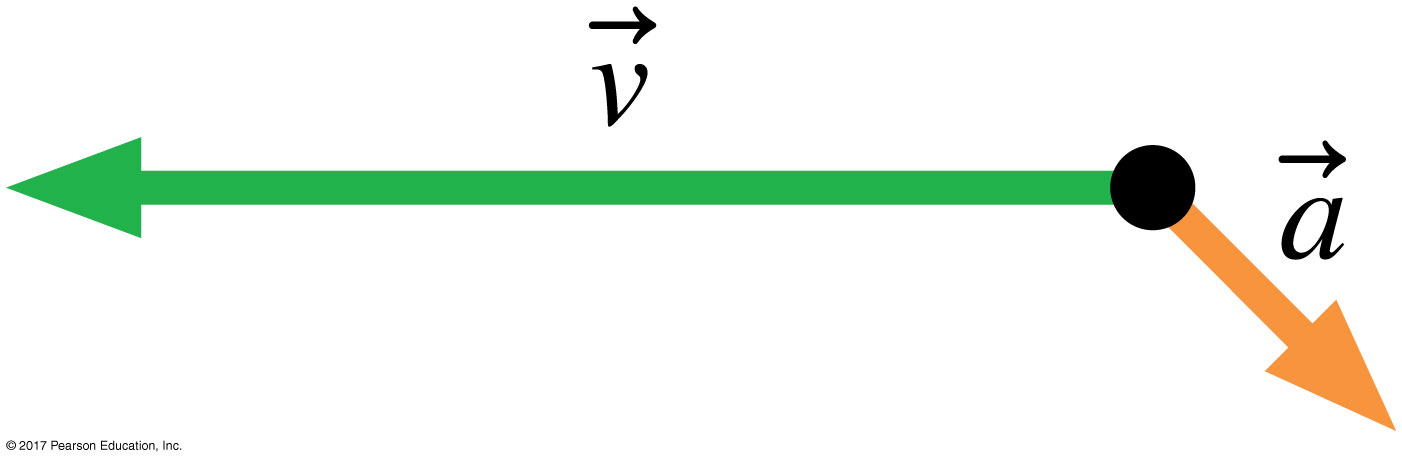
\includegraphics[width=0.5\textwidth]{../figures/Figure_STT4_2.jpg}
   \end{center}
   \begin{columns}
   \begin{column}{0.5\textwidth}
   \begin{enumerate}
      \item[A.] Speed up and curve upward
      \item[C.] Slow down and curve upward
      \item[E.] Move to the right and down
   \end{enumerate}
   \end{column}
   \begin{column}{0.55\textwidth}
   \begin{enumerate}
      \item[B.] Speed up and curve downward
      \item[D.] Slow down and curve downward
      \item[F.] Reverse direction
   \end{enumerate}
   \end{column}
   \end{columns}
\end{enumerate}
\end{frame}

\begin{frame}{Reminders}
\begin{itemize}
   \item HW is due on Saturday.
   \item The first exam is this coming Tuesday (19 Sep).
   \begin{itemize}
      \item Covers materials from chapters 1-4.
      \item Bring pencil and calculator. You cannot use a cell phone as a calculator as they need to be put away during the exam.
      \item You will get an hour to take the exam.
      \item We will have a question led review before the exam.
      \item Bring a standard sized notecard with any equaitons or information that you want on it. You can't share cards so make sure you bring your own!
   \end{itemize}
\end{itemize}
\end{frame}

\begin{frame}{Uniform Circular Motion}
\begin{itemize}
   \item What are some examples of circular motion?
   \begin{itemize}
      \item<2-> Ball on the end of a string being swung around
      \item<2-> Planet or Satellite orbiting a celestial object
      \item<2-> {\bf NOT} a spinning top, unless you're talking about a single point on the top.
   \end{itemize}
   \item<3-> If the {\it speed} around the circle is constant then the motion is called {\bf uniform circular motion}.
   \begin{center}
      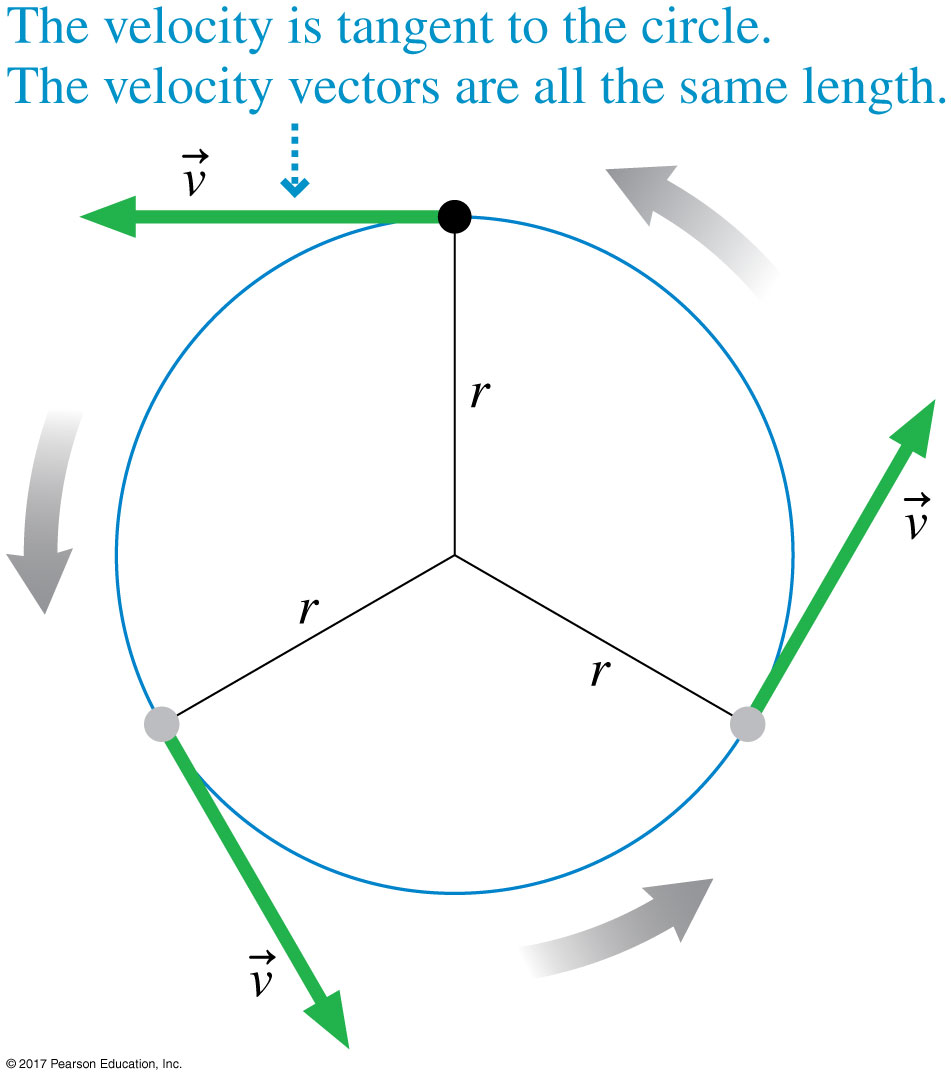
\includegraphics[width=0.4\textwidth]{../figures/04_21_Figure.jpg}
   \end{center}
\end{itemize}
\end{frame}

\begin{frame}{Uniform Circular Motion}
\begin{columns}
\begin{column}{0.4\textwidth}
   \begin{center}
      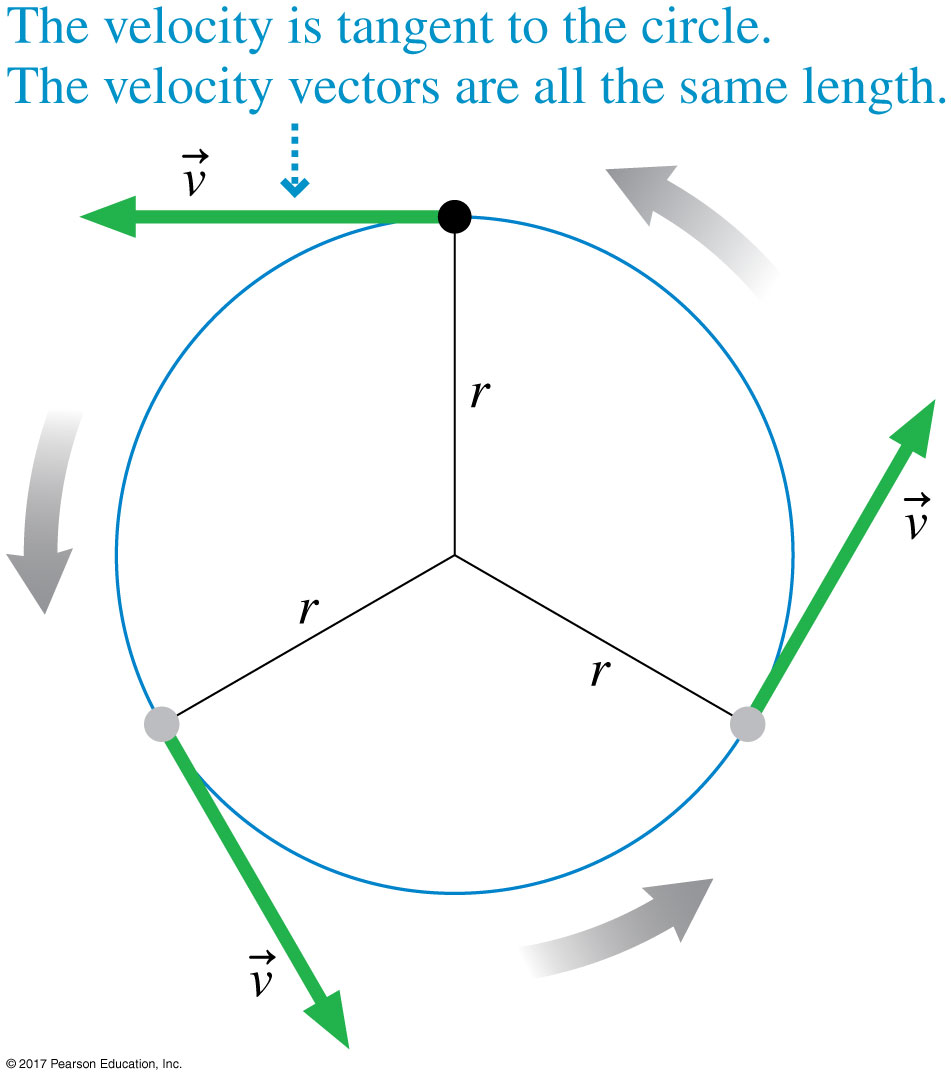
\includegraphics[width=\textwidth]{../figures/04_21_Figure.jpg}
   \end{center}
\end{column}
\begin{column}{0.6\textwidth}
   \begin{itemize}
      \item If the radius of motion is $r$ and the constant speed is $v$ then what is the {\bf period} of the motion?
      \item<2-> $v=\frac{1 \text{ circumference}}{1 \text{ period}} = \frac{2\pi r}{T}$
   \end{itemize}
\end{column}
\end{columns}
\end{frame}

\begin{frame}{Quick Check}
\begin{center}
   A 4.0-cm-diameter crankshaft turns at 2400 rpm (revolutions per minute). What is the speed of a point on the surface of the crankshaft?
   \begin{enumerate}
   \item<2-> Convert 2400 rpm to revolution per second
   \begin{equation*}
      \frac{2400 \text{ rev}}{1 \text{ min}} \times \frac{1 \text{ min}}{60 \text{ sec}} = 40 \text{ rev/sec}
   \end{equation*}
   \item<3-> How long it takes to do one turn is measured in seconds per revolution, s/rev
   \begin{equation*}
      T=\frac{1}{40}\text{ s} = 0.0025\text{ s}
   \end{equation*}
   \item<4-> Now plug in what we know to the equation we just found to get the speed
   \begin{equation*}
      v=\frac{2\pi r}{T} = \frac{2\pi(0.020\text{ m})}{0.025\text{ s}} = 5.0\text{ m/s}
   \end{equation*}
   \end{enumerate}
\end{center}
\end{frame}

\begin{frame}{Angular Position}
\begin{itemize}
   \item Which coordinates would be the easiest to use when describing the position vectors in circular motion, $(x,y)$ or $(r,\theta)$? Why?
   \begin{itemize}
      \item<2-> $r$ is often constant in circular motion and so the only thing that changes is $\theta$.
   \end{itemize}
\end{itemize}
\uncover<2>{\begin{center}
   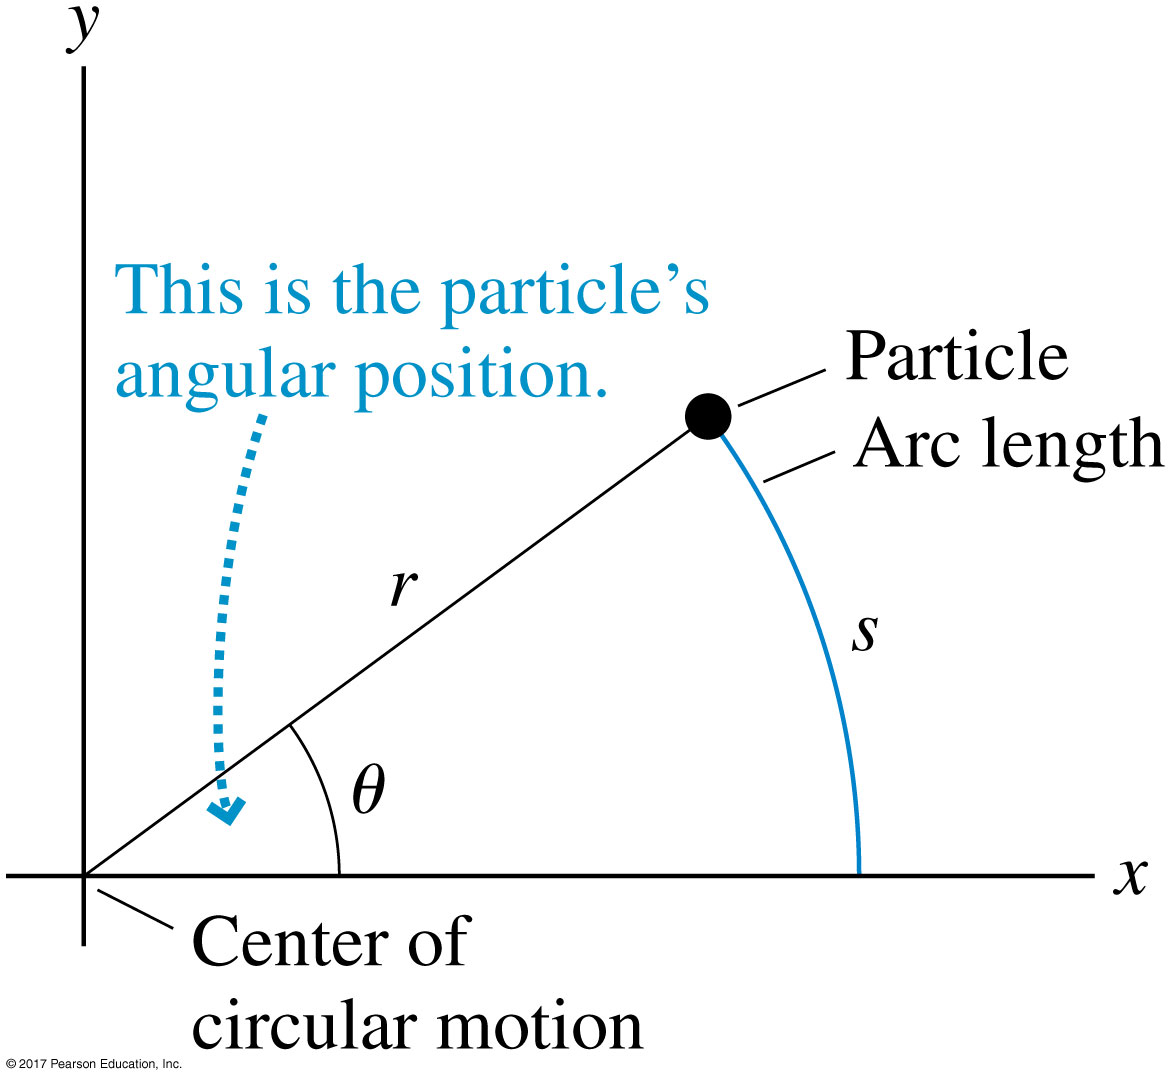
\includegraphics[width=0.5\textwidth]{../figures/04_22_Figure.jpg}
   ~\\ $\theta$ is called the {\bf angular position} of the particle.
\end{center}}
\end{frame}

\begin{frame}{Angular Position}
\begin{columns}
\begin{column}{0.4\textwidth}
   \begin{center}
      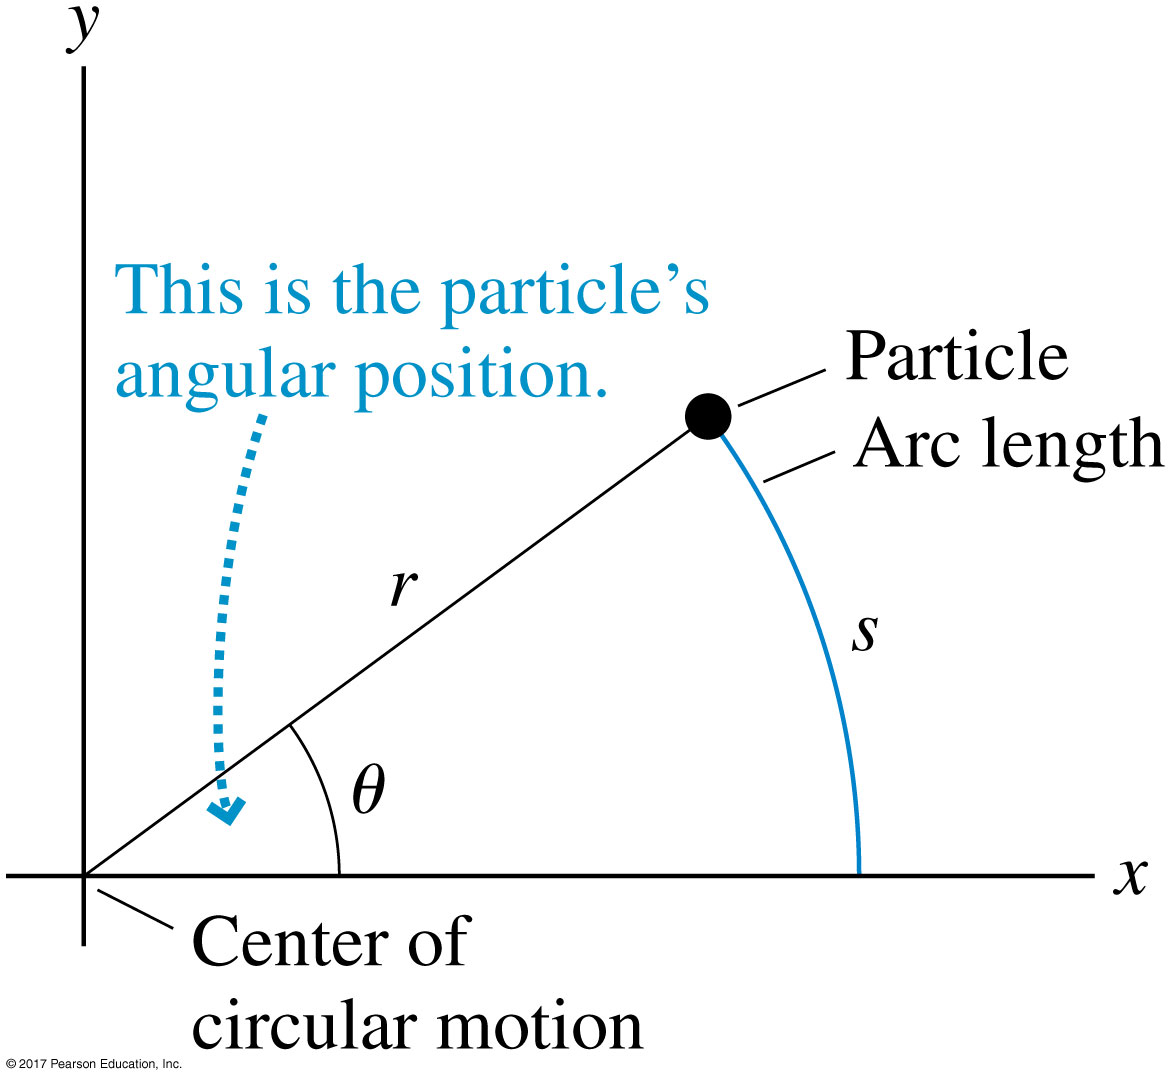
\includegraphics[width=\textwidth]{../figures/04_22_Figure.jpg}
   \end{center}
\end{column}
\begin{column}{0.6\textwidth}
   \begin{itemize}
      \item Angular position is defined (in radians) as
      \begin{equation*}
         \theta(\text{radians}) \equiv \frac{s}{r}
      \end{equation*}
      \item<1-> This is one of the reasons to use radians because $s=r\theta$ if $\theta$ is measured in radians.
   \end{itemize}
\end{column}
\end{columns}
~\\~
\begin{itemize}
   \item<2-> Radians are the SI unit for angle. How many radians are in a full circle?
   \begin{itemize}
      \item<3-> $\theta_{\text{full circle}} = \frac{2\pi r}{r} = 2\pi\text{ rad}$ ~~~~~~  1 rev = 360$^\circ$ = 2$\pi$ rad
   \end{itemize}
\end{itemize}
\end{frame}

\begin{frame}{Quick Check}
\begin{center}
   Convert 1 rad to degrees? \\
   \uncover<2>{\begin{equation*}
      1\text{ rad} = 1\text{ rad} \times \frac{360^\circ}{2\pi\text{ rad}} = 57.3^\circ
   \end{equation*}
   ~\\ Note that 1 rad is $\approx$ 60$^\circ$, this can make quick calculations easier to do in your head.}
\end{center}
\end{frame}


\begin{frame}{Angular Velocity}
\begin{center}
   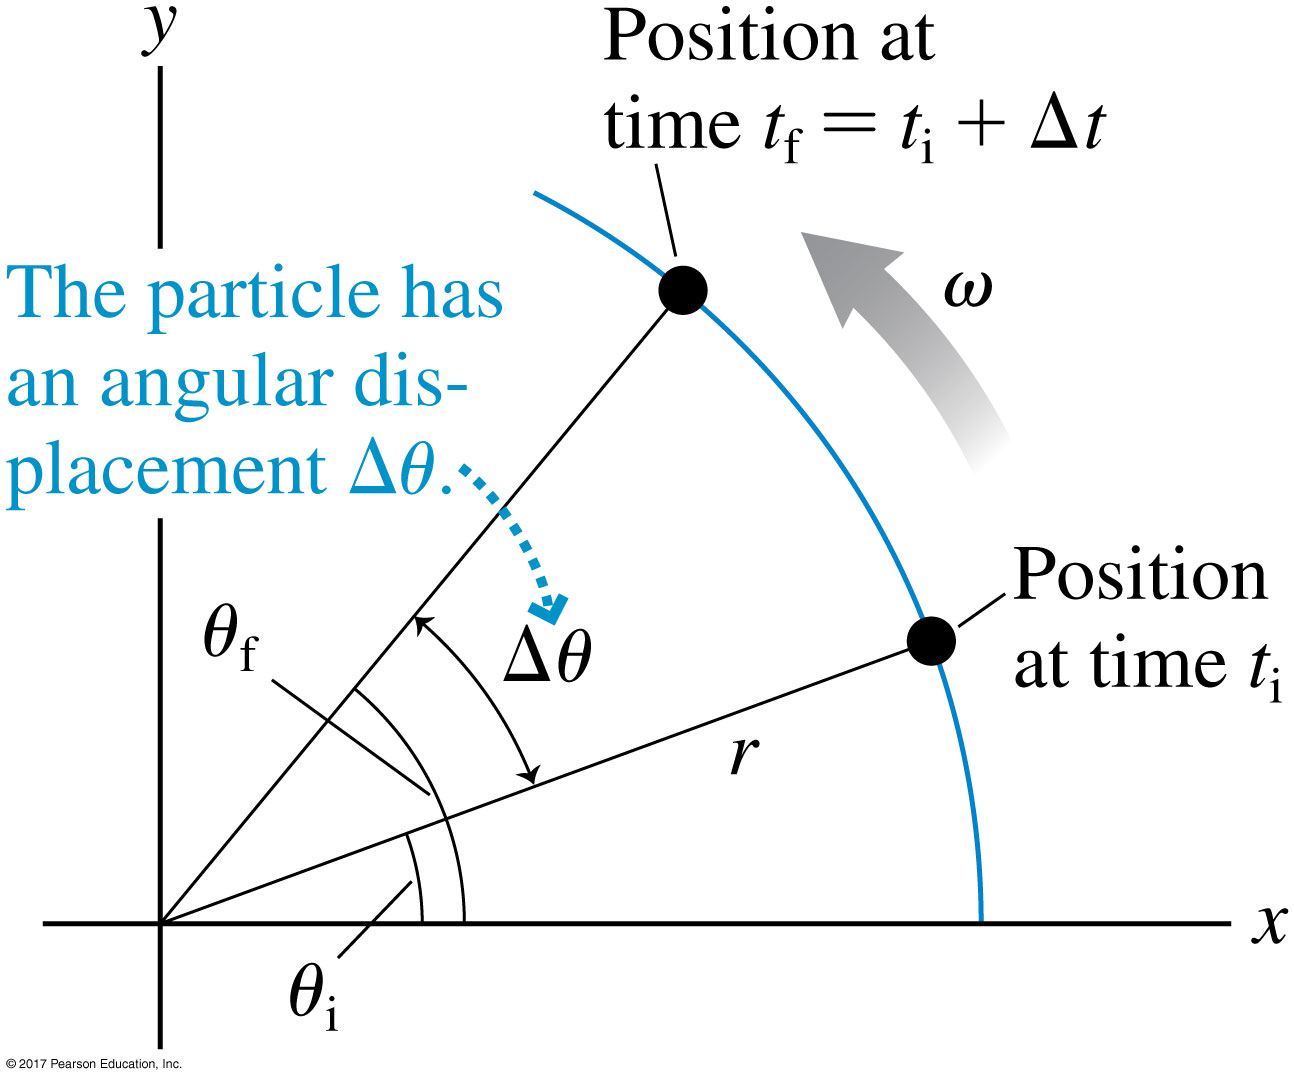
\includegraphics[width=0.4\textwidth]{../figures/04_23_Figure.jpg}
\end{center}
\begin{itemize}
   \item We can define an {\it angular} displacement, $\Delta\theta$ (just like $\Delta r$) just like we did before.
   \item<2-> From this we can define an average {\bf angular velocity}
   \begin{equation*}
      \text{angular velocity} = \omega \equiv \frac{\Delta\theta}{\Delta t},
   \end{equation*}
   which is the rate at which the angular position changes with respect to time \\ *$\omega$ is the Greek leter ``omega" not just w
\end{itemize}
\end{frame}

\begin{frame}{Angular Velocity}
\begin{itemize}
   \item How do you know if $\omega$ is positive or negative? (think right hand rule)
\end{itemize}
\begin{center}
\uncover<2>{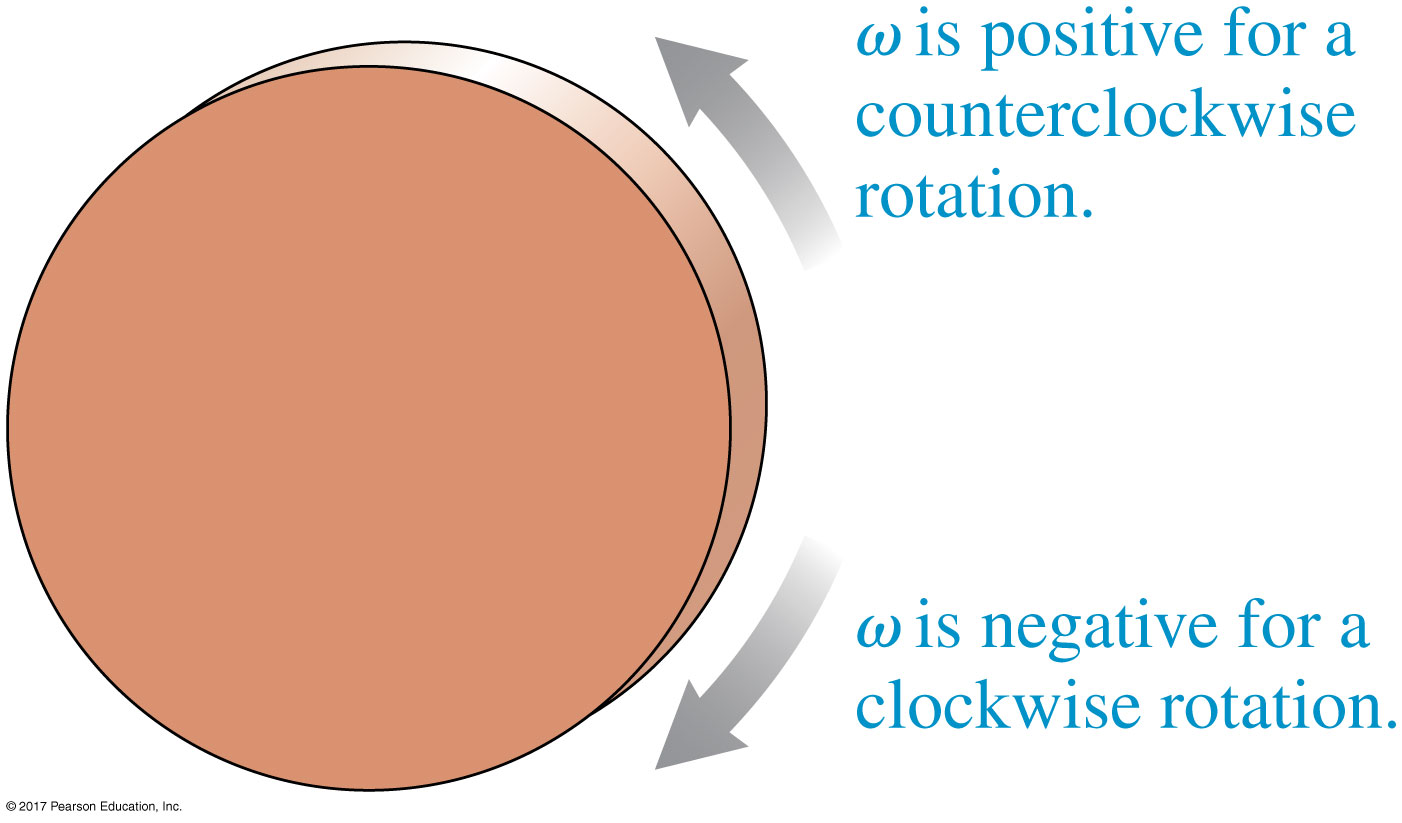
\includegraphics[width=0.4\textwidth]{../figures/04_24_Figure.jpg}}
\end{center}
\begin{itemize}
   \item<3-> So if we have uniform circular motion what does that tell us about $\omega$?
   \begin{itemize}
      \item<4-> Uniform circular motion means that $\omega$ is constant (just like uniform motion meant that $v$ was constant).
   \end{itemize}
\end{itemize}
\end{frame}

\begin{frame}{Angular Velocity}
\begin{itemize}
   \item Just as before if we take the limit of the average angular velocity you get a derivative
\end{itemize}
\begin{equation*}
   \omega \equiv \lim\limits_{\Delta t\rightarrow 0} \frac{\Delta\theta}{\Delta t} = \frac{d\theta}{dt}
\end{equation*}
\begin{itemize}
   \item<2-> Since everything for $\omega$ and $\theta$ parallel $s$ and $v$ we can draw some general conclusions about the graphical representations.
   \begin{itemize}
      \item<2-> $\omega = $ slope of the $\theta$-versus-$t$ graph at time $t$
      \item<2-> $\theta_f = \theta_i + $ area under the $\omega$-versus-$t$ curve between $t_i$ and $t_f$ = $\theta_i + \omega\Delta t$
   \end{itemize}
\end{itemize}
\end{frame}

\begin{frame}{Quick Check}
\begin{center}
   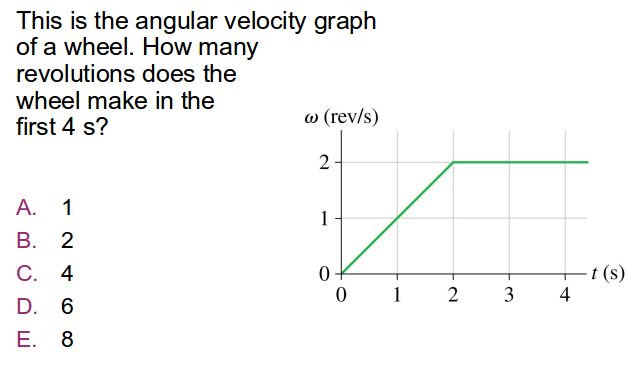
\includegraphics[width=\textwidth]{../figures/QC4_7.png}
\end{center}
\only<2>{\checkL{0.9cm}{6.5cm}}
\end{frame}

\begin{frame}{Angular Velocity}
\begin{itemize}
   \item The angular velocity and period are related, can you figure out how?
   \item<2-> The period is the time it takes to do one full revolution (i.e. $\Delta\theta=2\pi$ rad). So we get
\end{itemize}
\uncover<2>{\begin{equation*}
   \left|\omega\right| = \frac{2\pi\text{ rad}}{T} ~~\rightarrow~~ T = \frac{2\pi\text{ rad}}{\left|\omega\right|}
\end{equation*}}
\end{frame}

\begin{frame}{Quick Check}
\begin{center}
   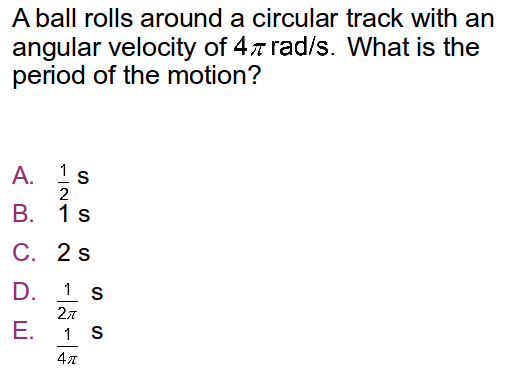
\includegraphics[width=\textwidth]{../figures/QC4_8.png}
\end{center}
\only<2>{\checkL{0.9cm}{4.3cm}}
\end{frame}

\begin{frame}{Tangential Velocity}
\begin{center}
   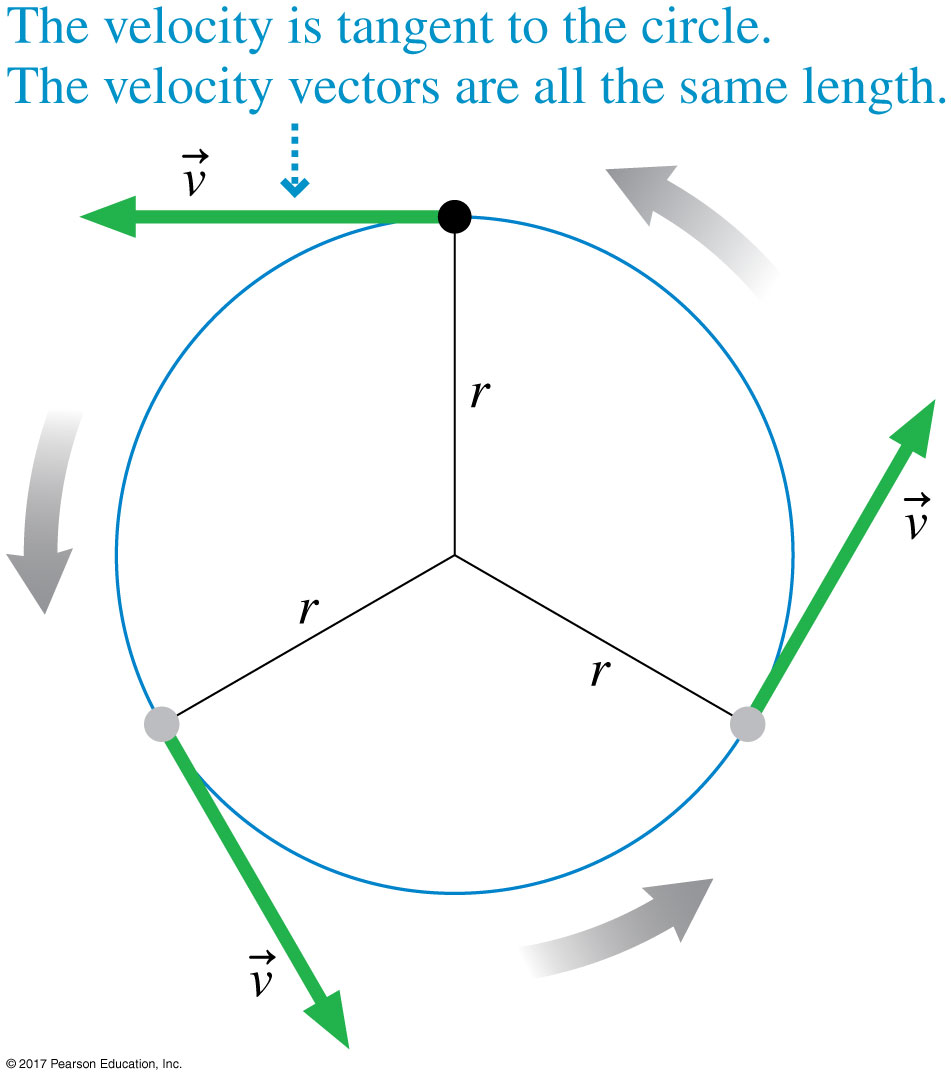
\includegraphics[width=0.3\textwidth]{../figures/04_21_Figure.jpg}
\end{center}
\begin{itemize}
   \item The {\bf tangential velocity} of an object is the speed at which the object moves around the circle, $ds/dt$, where $s$ is the arc length.
   \item<2-> Just like arc length could be described in terms of the angle (in radians) the tangential velocity can be descrived in terms of the angular momentum (in rad/s).
\end{itemize}
\uncover<2>{\begin{equation*}
   v_t = \omega r
\end{equation*}}
\end{frame}

\begin{frame}{Quick Check}
\begin{center}
   A particle moves cw around a circle at constant speed for 2.0 s. It then reverses direction and moves ccw at half the original speed until it has traveled through the same angle. Which is the particle's angle-versus-time graph? \\~\\
   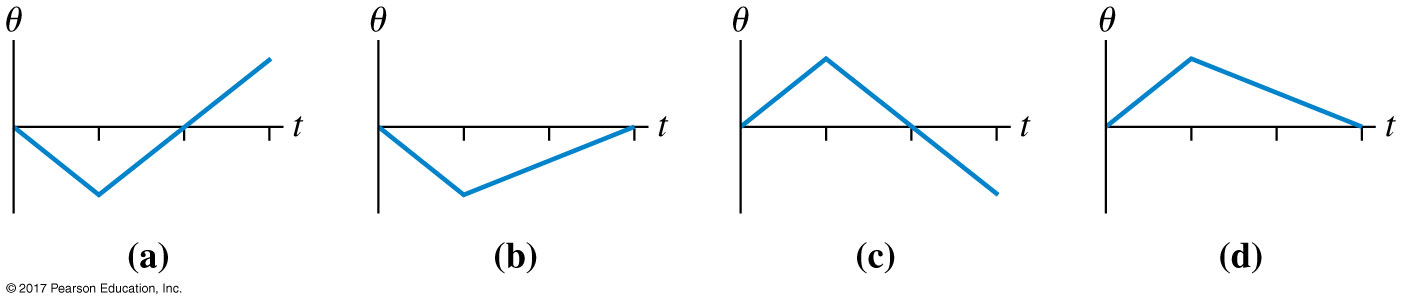
\includegraphics[width=\textwidth]{../figures/Figure_STT4_5.jpg}
\end{center}
\only<2>{\checkl{5.0cm}{6.5cm}}
\end{frame}

\begin{frame}{Centripital Acceleration}
\begin{columns}
\begin{column}{0.4\textwidth}
\begin{center}
   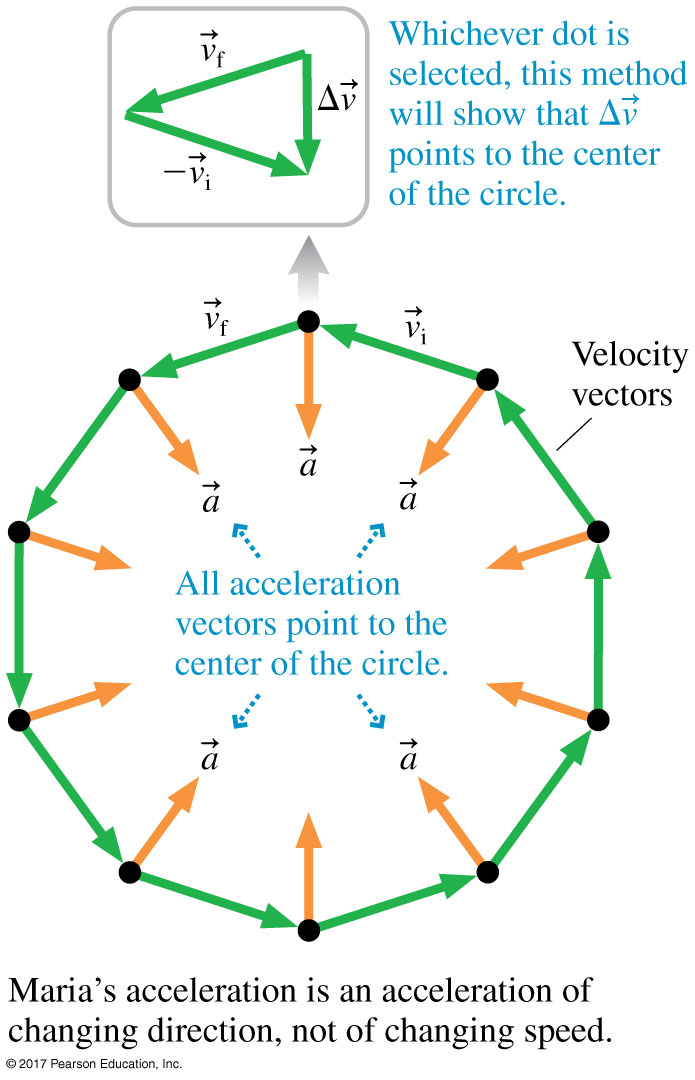
\includegraphics[width=\textwidth]{../figures/04_27_Figure.jpg}
\end{center}
\end{column}
\begin{column}{0.6\textwidth}
\begin{itemize}
   \item This is the motion of a car on a ferris wheel.
   \item The acceleration direction is always pointing to the center. This is {\bf centripital acceleration} (Greek for ``center seeking")
   \item This is the acceleration of uniform circular motion.
   \item The magnitude of $a_c$ is $v^2/r$, where $v$ is the tangential velocity.
\end{itemize}
\begin{shaded}
\begin{equation*}
   \vec{a}_c = \left(\frac{v^2}{r}, \text{ toward center of circle}\right)
\end{equation*}
\end{shaded}
\end{column}
\end{columns}
\end{frame}

\begin{frame}{Quick Check}
\begin{center}
   Rank in order, from largest to smallest, the centripetal accelerations of these particles.
   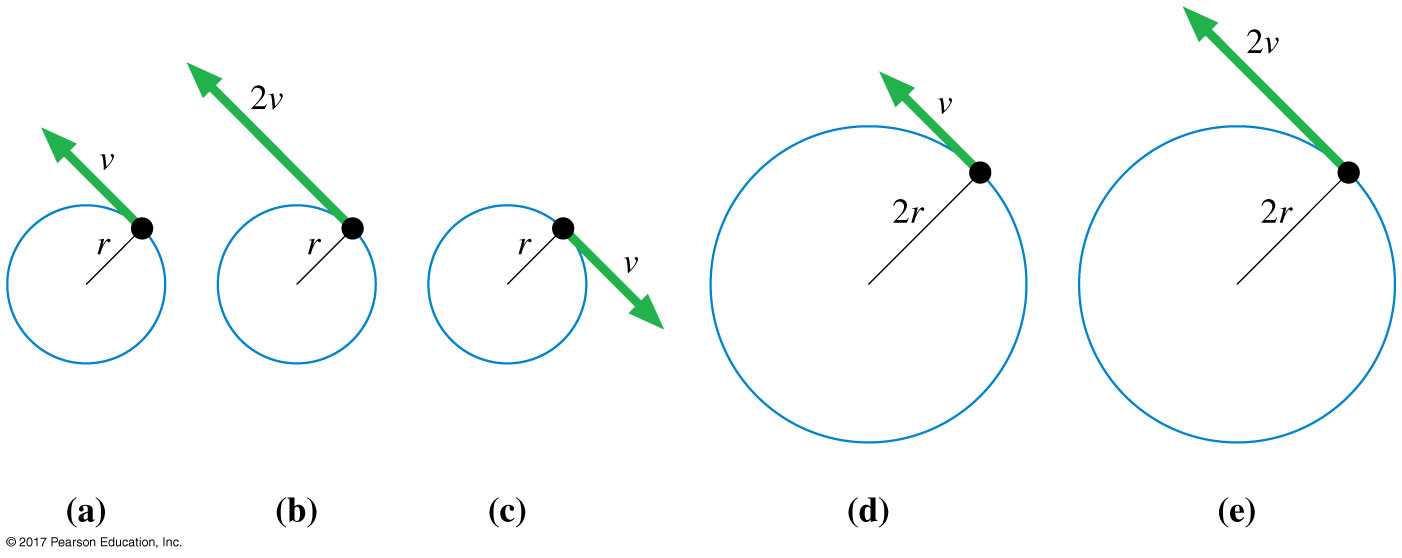
\includegraphics[width=\textwidth]{../figures/Figure_STT4_6.jpg}
   \uncover<2>{\\~\\ b,e,(a,c),d}
\end{center}
\end{frame}

\begin{frame}{Quick Check}
\begin{center}
   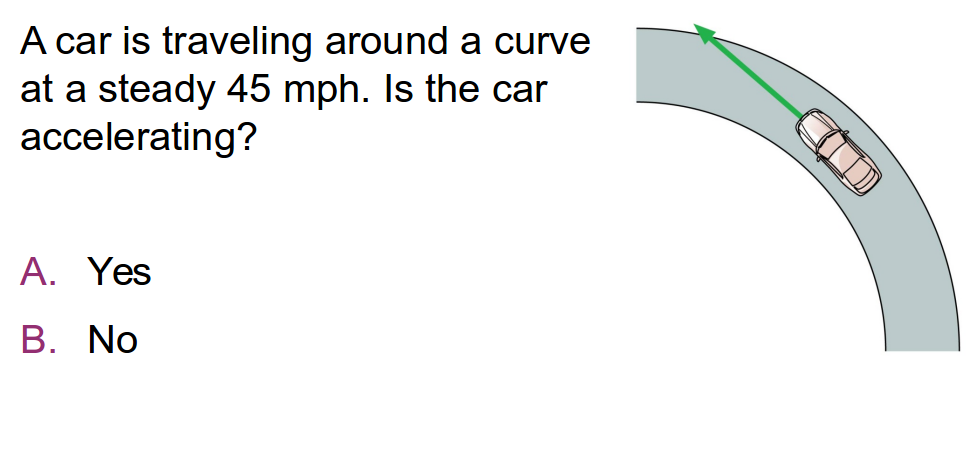
\includegraphics[width=\textwidth]{../figures/QC4_9.png}
\end{center}
\only<2>{\checkh{0.7cm}{4.7cm}}
\end{frame}

\begin{frame}{Quick Check}
\begin{center}
   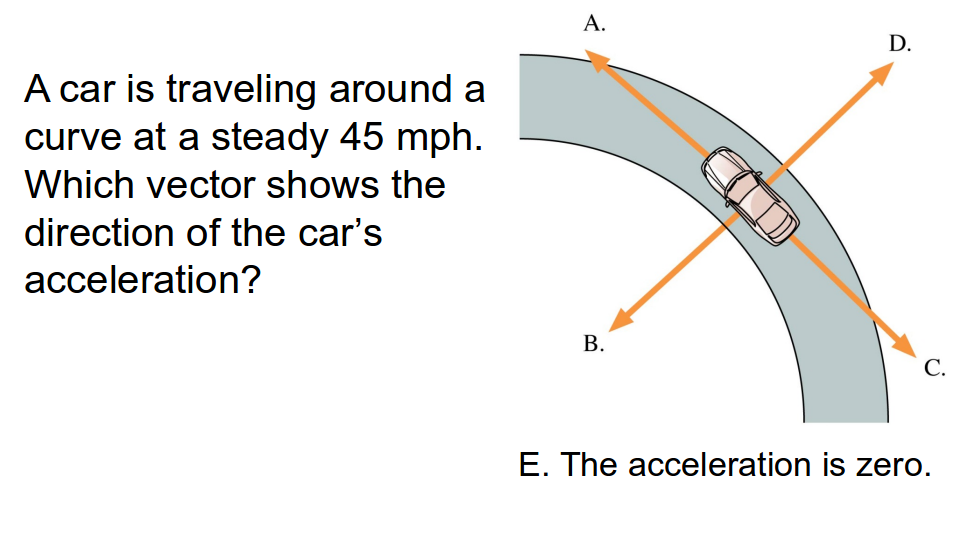
\includegraphics[width=\textwidth]{../figures/QC4_10.png}
\end{center}
\only<2>{\checkh{7.4cm}{5.3cm}}
\end{frame}

\begin{frame}{Quick Check}
\begin{center}
   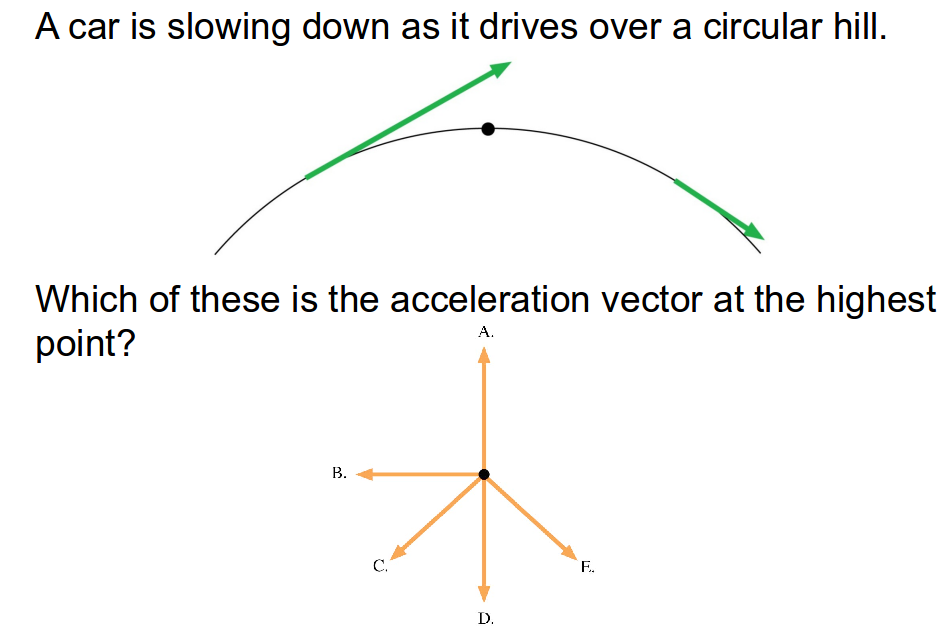
\includegraphics[width=\textwidth]{../figures/QC4_11.png}
\end{center}
\only<2>{\checkl{5.4cm}{7.4cm}}
\end{frame}

\begin{frame}{Angular Acceleration}
\begin{itemize}
   \item If an object is speeding up as it is going about it's circular orbit (like a car speeding around a turn or a roller coaster slowing down then speeding up on a loop) this motion is called {\bf nonlinear circular motion}.
   \item<2-> The angular acceleration (rate of change of $\omega$) is given the Greek symbol alpha and is defined as you might imagine
\end{itemize}
\uncover<2>{\begin{equation*}
   \alpha \equiv \frac{d\omega}{dt}
\end{equation*}}
\begin{itemize}
   \item<3-> The units for $\alpha$ are rad/s$^2$ and you need to remember that the sign doesn't mean slowing down or speeding up.
\end{itemize}
\begin{center}
   \uncover<3>{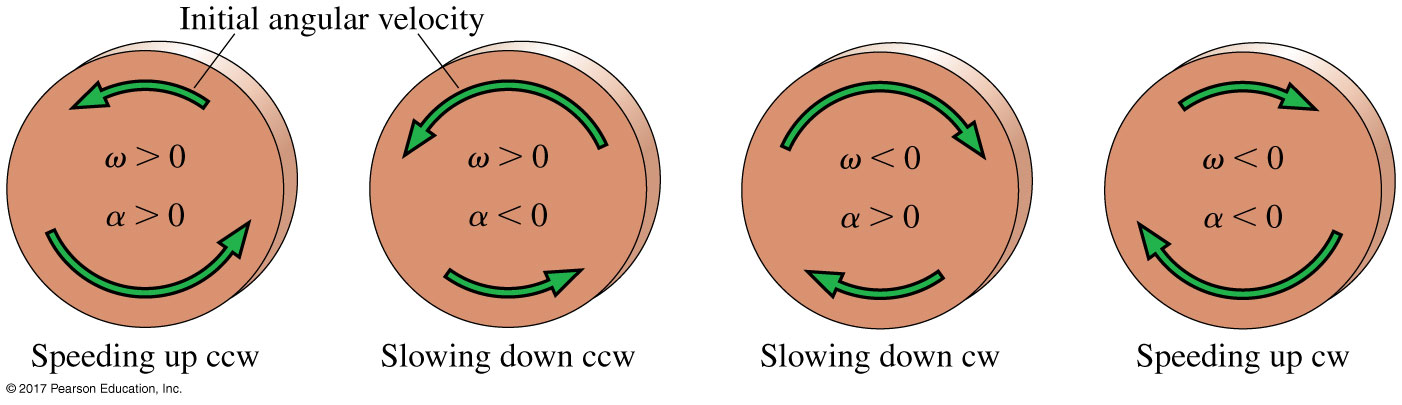
\includegraphics[width=\textwidth]{../figures/04_30_Figure.jpg}}
\end{center}
\end{frame}

\begin{frame}{Angular Acceleration}
\begin{center}
   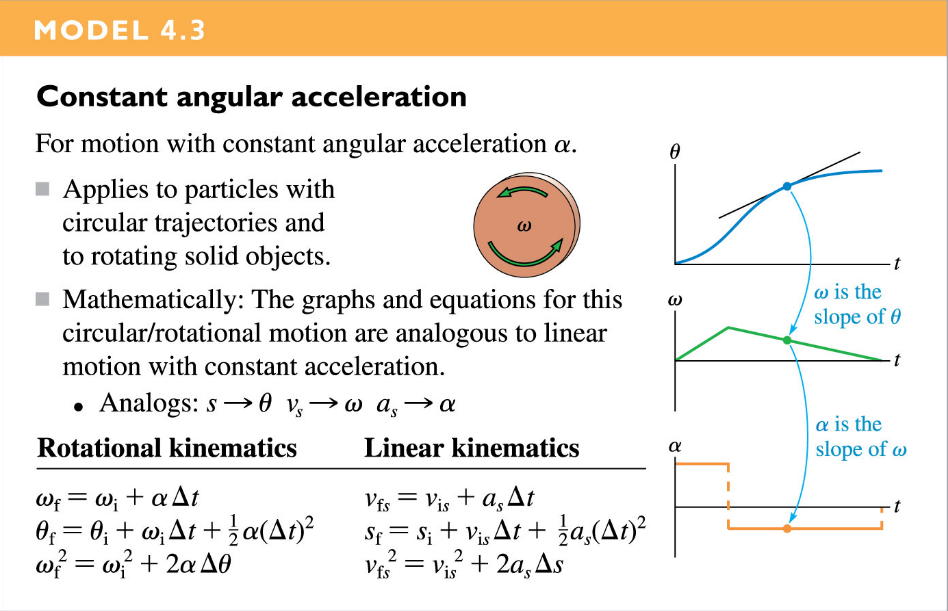
\includegraphics[width=\textwidth]{../figures/model4_3.png}
\end{center}
\end{frame}

\begin{frame}{Quick Check}
\begin{center}
   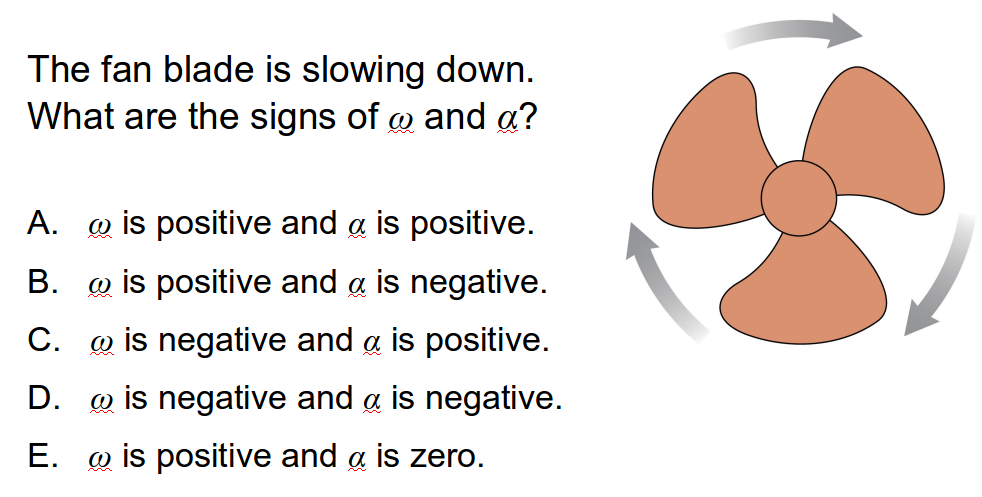
\includegraphics[width=\textwidth]{../figures/QC4_15.png}
\end{center}
\only<2>{\checkl{0.8cm}{5.4cm}}
\end{frame}

\begin{frame}{Tangential Acceleration}
\begin{columns}
\begin{column}{0.4\textwidth}
\begin{center}
   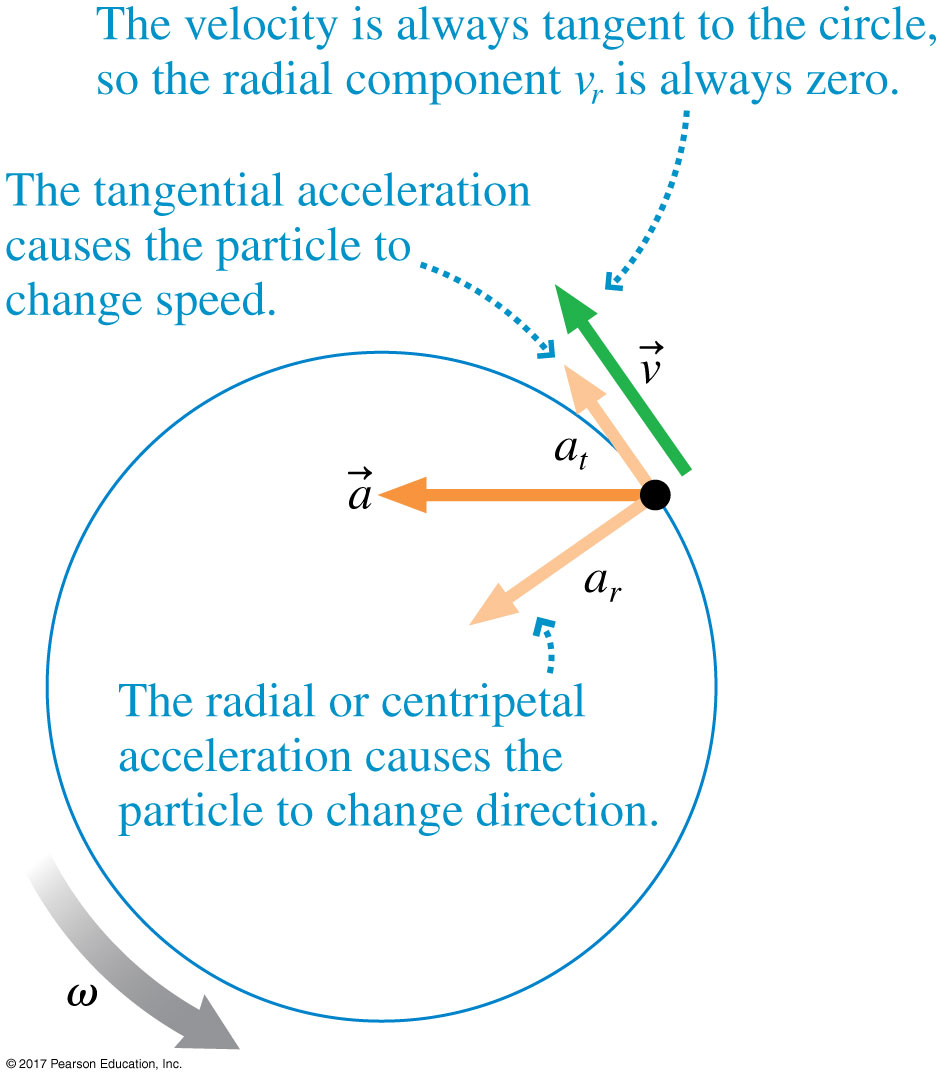
\includegraphics[width=\textwidth]{../figures/04_32_Figure.jpg}
\end{center}
\end{column}
\begin{column}{0.6\textwidth}
\begin{itemize}
   \item Just like with velocity we can define a {\bf tangential acceleration}.
   \item This is the same as the parralel part of the acceleration, the part that causes it to change speed, $\vec{a}_\parallel = \vec{a}_t$.
   \item<2-> That means that the perpendicular part is the {\bf radial acceleration} (similar to centripital for uniform circular motion), $\vec{a}_\perp = \vec{a}_r = v_t^2/r = \omega^2/r$.
   \item<3-> The magnitude of a is given by $a=\sqrt{a_r^2+at^2}$.
   \item<4-> And just like with $v_t$ we can write $a_t = \alpha r$.
\end{itemize}
\end{column}
\end{columns}
\end{frame}

\begin{frame}{Picture References}
\tiny
None yet
\end{frame}

\end{document}
